\documentclass{standalone}
\usepackage{pgf,tikz}
%\usepackage{mathrsfs}
\usetikzlibrary{arrows}
\pagestyle{empty}
\begin{document}
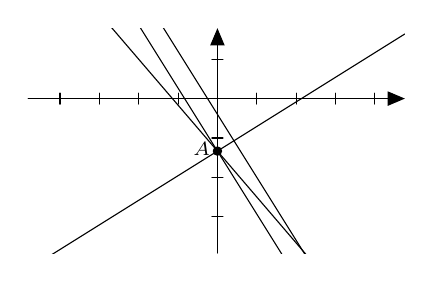
\begin{tikzpicture}[line cap=round,line join=round,>=triangle 45,x=1.0cm,y=1.0cm]
\draw[->,color=black] (-2.4028860620261123,0.) -- (2.380414521398098,0.);
\foreach \x in {-2.,-1.5,-1.,-0.5,0.5,1.,1.5,2.}
\draw[shift={(\x,0)},color=black] (0pt,2pt) -- (0pt,-2pt);
\draw[->,color=black] (0.,-1.9633227313681136) -- (0.,0.8936418347859234);
\foreach \y in {-1.5,-1.,-0.5,0.5}
\draw[shift={(0,\y)},color=black] (2pt,0pt) -- (-2pt,0pt);
\clip(-2.4028860620261123,-1.9633227313681136) rectangle (2.380414521398098,0.8936418347859234);
\draw [domain=-2.4028860620261123:2.380414521398098] plot(\x,{(-4.-7.*\x)/6.});
\draw [domain=-2.4028860620261123:2.380414521398098] plot(\x,{(-1.-8.*\x)/5.});
\draw [domain=-2.4028860620261123:2.380414521398098] plot(\x,{(-32.--30.*\x)/48.});
\draw [domain=-2.4028860620261123:2.380414521398098] plot(\x,{(-20.-48.*\x)/30.});
\begin{scriptsize}
\draw [fill=black] (0.,-0.6666666666666666) circle (1.5pt);
\draw[color=black] (-0.2,-0.6422206654700053) node {$A$};
\end{scriptsize}
\end{tikzpicture}
\end{document}